\section{Definición de problema}

Definición de variables y parámetros para \textit{route selection for emergency logistics management}:
\begin{itemize}
		\item $l_{ij}$ denota el largo de los arcos que se encuentra entre los nodos $v_i$ y $v_j$, donde $(v_i,v_j) \in A$.
	\item $s_{ij}^0$ es la velocidad entre los arcos $(v_i,v_j)$ en condiciones normales. Sea $s_{ij}(t)$ es la velocidad de viaje en el arco $(v_i,v_j)$ bajos las condiciones del desastre en el tiempo t.\\

\begin{figure}[h]
\centering
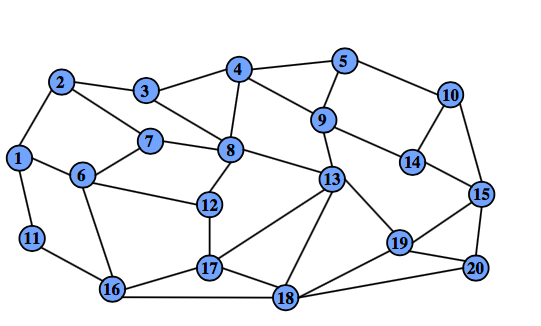
\includegraphics[scale=0.5]{images/routes.png}
\caption{Estructura de una red de emergencia}
\end{figure}
	
    A partir de la observación de desastres como huracanes e inundaciones Se afirma que la velocidad de viaje en cada arco de la red decrece con el impacto del desastre \cite{tufekci1995integrated}. La disminución de la velocidad de viaje es dependiente de la posición del arco, el tipo de desastre y otros.  Sin pérdida de generalidad, la función de velocidad puede representarse como:
\begin{equation}
	  s_{ij}(t) = s_{ij}^0 \cdot \alpha_{ij} \cdot e^{-\beta_{ij} \cdot t}
\end{equation}
donde \(\alpha_{ij}\) y \(\beta_{ij}\) son los parámetros decrecientes que determinan la disminución de la velocidad del viaje \(s_{ij}(t)\), \(\alpha_{ij}\) y \(\beta_{ij}\) pueden ser estimados de acuerdo a factores como la distancia desde arco $(v_i,v_j)$ al centro del desastre, la vulnerabilidad del arco, el tipo de desastre, entre otros.
	\item Sea \(t_{ij}\) el tiempo necesario para viajar a través del arco $(v_i,v_j)$, se calcula como $t_{ij}=t_j-t_i$.
	\item Sea $x_{ij}$ es variable de decisión del modelo $x_{ij} = 1 $ cuando el arco $(v_i,v_j)$ es incluido en el camino y $x_{ij} = 0 $ cuando el arco $(v_i,v_j)$ no es incluido en el camino.
	\item P denota el camino realizado, o sea la secuencia de nodos en la redes que se elige. Sea $p_k$ el número de la secuencia del nodo $v_{p_k}$	en la red, entonces P puede ser presentado como $(v_{p_1},v_{p_2},\cdots,v_{p_k},\cdots,v_{p_K})$ donde $1\leq p_k \leq n$ y k es la secuencia del nodo   $v_{p_k}$ en el camino P.  P debe iniciar en el nodo inicial $p_1=1$ y $p_K=n$. Y no deben existir ciclos.
	\item Sea $ET(P,v_{p_k})$ el tiempo de viaje desde $v_{p_1}$ que termina en $v_{p_k}$ a lo largo de $(v_{p_1},v_{p_2},\cdots,v_{p_k})$ donde $1\leq p_k \leq n$. A partir de esto se determina que:
	\begin{equation}
		ET(P,v_{p_k})= \sum_{m=1}^{k-1} t_{p_mp_{m+1}} = (t_{p_2} - t_{p_1}) +(t_{p_3} - t_{p_2}) + \cdots + (t_{p_k} - t_{p_{k-1}}) = t_{p_k}
	\end{equation}
	

\end{itemize}
 A partir de lo anterior podemos calcular el tiempo de un camino, dado que:
\begin{equation}\label{borde}
	  t_{p_1} = t_1 = 0
\end{equation} 
 
\begin{equation}\label{int}
\int_{t_{p_{k-1}}}^{t_{p_k}} s_{p_{k-1}p_k}(t)dt = l_{p_{k-1}p_k} \text{  \(2 \leq k \leq  K\)}
 \end{equation}
 
En la ecuación \eqref{int} conocemos el límite inferior de la integral, el integrando $ s_{p_{k-1}p_k}$ y el resultado de $ l_{p_{k-1}p_k} $, por lo tanto, se puede obtener el límite superior $t_{p_k}$.
Por recursividad se puede obtener los valores de $t_{p_k}$ para los nodos $v_{p_k}$ con  $1\leq p_k \leq n$.

\subsection{Modelo matemático}
%Uno o m\'as modelos matem\'aticos para el problema, idealmente indicando elp espacio de b\'usqueda para cada uno.
A continuación se resume la notación utilizada para modelar el problema \textit{route selection for emergency logistics management}
\subsubsection{Notación}
\begin{itemize}
	\item $i$  indice para los nodos en la red
	\item $v_i$ nodo $i$ de la red
 	\item $(i,j)$ arco desde i a j
	\item $x_{ij}$ variable de decisión del modelo, $x_{ij} = 1 $ cuando el arco de los nodos $(v_i,v_j)$ es incluido en el camino, en caso contrario $x_{ij} = 0$
	\item $l_{ij}$ largo del arco desde i a j
	\item $s^{o}_{ij}$  velocidad entre los arcos $(v_i, v_j)$ en condiciones normales
	\item $s_{ij}(t)$ velocidad entre los arcos $(v_i, v_j)$ en el tiempo $t$
	\item $\alpha_{ij}$ parámetro decreciente para manipular la velocidad           
	\item $\beta_{ij}$ parámetro decreciente para manipular la velocidad             
	\item $t_{ij}$ tiempo necesario para viajar entre i y j                      
\end{itemize}

Considerando lo descrito por \cite{southworth1991regional,cova2003network} se diseñan dos modelos con distintos objetivos: el primero busca la minimización del tiempo y el segundo busca múltiples objetivos: la minimización del tiempo y de la cantidad de nodos en la ruta.
\subsubsection{Minimización del tiempo:} 

La formulación del \textit{route selection for emergency logistics management} se describe de la siguiente manera:

El objetivo del modelo es minimizar el tiempo empleado en el camino. Las ecuaciones \eqref{7}, \eqref{8} y \eqref{9} son parte de la fórmula de recursión del tiempo total para el camino. En la ecuación \eqref{speed} la función decreciente de la velocidad de viaje en el arco $(v_i,v_j)$. La restricción \eqref{full} asegura un camino factible desde $v_1$ hasta $v_n$ y la restricción \eqref{circles} asegura que no existan ciclos.

\begin{equation}
	 \text{mín} \sum_{i=1}^{n}\sum_{j=1}^{n} t_{ij} \cdot x_{ij}
\end{equation}

\begin{equation}\label{7}
  \int_{t_i}^{t_j} s_{ij}(t)dt = l_{ij}
\end{equation}
\begin{equation}\label{8}
  t_{ij} = t_j - t_i
\end{equation}
\begin{equation}\label{9}
t_1 =0
\end{equation}
\begin{equation}\label{speed}
  s_{ij}(t) = s_{ij}^0 \cdot \alpha_{ij} \cdot e^{-\beta_{ij}\cdot t}
\end{equation}

\begin{equation}\label{full}
	\sum_{\substack{j=1\\
                  j \neq i}}^n x_{ij} - \sum_{\substack{j=1\\
                  j \neq i}}^{n} x_{ji} = \begin{cases}
1 & i=1\\
-1 & i=n \\
0 & eoc
\end{cases}
\end{equation}



\begin{equation}\label{circles}
	\sum_{\substack{j=1\\
                  j \neq i}}^n x_{ij} = \begin{cases}
\leq 1 & i\neq n\\
=0 & i=n 
\end{cases}
\end{equation}

\begin{equation}
	x_{ij} = 0,1;i=1,2,\cdots,n;j=1,2,\cdots,n
\end{equation}

%\subsubsection{Multi-objetivo para \textit{route selection for emergency logistics management} }
%
%\cite{southworth1991regional,cova2003network} han mostrado que la mayor congestión sucede en las intersecciones de dos arcos en una red de emergencia, cuando se viaja en un camino con menor número de arcos es más fácil y rápido seguir el camino. La complejidad del camino puede obtenerse por el número de arcos incluídos en un camino. 
%
%
%\begin{equation}\label{f_1}
%	 \text{mín}  f_1 = \sum_{i=1}^{n}\sum_{j=1}^{n} t_{ij}x_{ij}
%\end{equation}
%
%
%\begin{equation}\label{f_2}
%	 \text{mín}  f_2 = \sum_{i=1}^{n}\sum_{j=1}^{n} x_{ij}
%\end{equation}
%
%Las restricciones se heredan del modelo anterior.